\documentclass[aspectratio=169,t]{beamer}

\usepackage{xcolor}
\definecolor{darkbg}{HTML}{0D1117}
\definecolor{slidebg}{HTML}{161B22}
\definecolor{accent}{HTML}{58A6FF}
\definecolor{accentgreen}{HTML}{3FB950}
\definecolor{accentorange}{HTML}{F78166}
\definecolor{accentyellow}{HTML}{E3B341}
\definecolor{textprimary}{HTML}{E6EDF3}
\definecolor{textsecondary}{HTML}{8B949E}
\definecolor{blockbg}{HTML}{21262D}
\definecolor{firered}{HTML}{E94560}
\definecolor{fireorange}{HTML}{FF6B35}

\setbeamercolor{background canvas}{bg=darkbg}
\setbeamercolor{normal text}{fg=textprimary}
\setbeamercolor{frametitle}{fg=accent,bg=slidebg}
\setbeamercolor{title}{fg=accent}
\setbeamercolor{subtitle}{fg=textsecondary}
\setbeamercolor{author}{fg=textprimary}
\setbeamercolor{date}{fg=textsecondary}
\setbeamercolor{footline}{fg=textsecondary,bg=slidebg}
\setbeamercolor{section in toc}{fg=textprimary}
\setbeamercolor{itemize item}{fg=accent}
\setbeamercolor{itemize subitem}{fg=accentgreen}
\setbeamercolor{itemize subsubitem}{fg=accentyellow}
\setbeamercolor{enumerate item}{fg=accent}
\setbeamercolor{enumerate subitem}{fg=accentgreen}
\setbeamercolor{block title}{fg=accent,bg=blockbg}
\setbeamercolor{block body}{fg=textprimary,bg=blockbg}
\setbeamercolor{block title alerted}{fg=firered,bg=blockbg}
\setbeamercolor{block body alerted}{fg=textprimary,bg=blockbg}
\setbeamercolor{block title example}{fg=accentgreen,bg=blockbg}
\setbeamercolor{block body example}{fg=textprimary,bg=blockbg}

\setbeamertemplate{navigation symbols}{}
\setbeamertemplate{frametitle}[default][left]
\setbeamertemplate{itemize item}{\textbullet}
\setbeamertemplate{itemize subitem}{$\circ$}
\setbeamerfont{frametitle}{size=\large,series=\bfseries}
\setbeamerfont{title}{size=\LARGE,series=\bfseries}

\setbeamertemplate{footline}{%
  \begin{beamercolorbox}[wd=\paperwidth,ht=2.5ex,dp=1ex,leftskip=3mm,rightskip=3mm]{footline}%
    \scriptsize \textcolor{textsecondary}{Wildfire Detection CNN}\hfill
    \textcolor{textsecondary}{\insertframenumber{} / \inserttotalframenumber}
  \end{beamercolorbox}%
}

\usepackage{amsmath,amssymb,amsfonts}
\usepackage{booktabs}
\usepackage{array}
\usepackage{tikz}
\usetikzlibrary{shapes,arrows,positioning,fit,calc}
\usepackage{graphicx}
\usepackage{colortbl}
\usepackage{adjustbox}

\setbeamersize{text margin left=6mm, text margin right=6mm}
\setbeamerfont{block title}{size=\normalsize}
\setbeamerfont{block body}{size=\small}

% TikZ named styles (no parameters - avoids beamer hash issues)
\tikzset{
  tbox/.style={rectangle, rounded corners=2pt, draw=accent, fill=accent!15,
               text=black, minimum width=1.6cm, minimum height=0.5cm,
               font=\scriptsize, align=center},
  tboxg/.style={rectangle, rounded corners=2pt, draw=accentgreen, fill=accentgreen!15,
               text=black, minimum width=1.6cm, minimum height=0.5cm,
               font=\scriptsize, align=center},
  tboxr/.style={rectangle, rounded corners=2pt, draw=firered, fill=firered!15,
               text=black, minimum width=1.6cm, minimum height=0.5cm,
               font=\scriptsize, align=center},
  tboxo/.style={rectangle, rounded corners=2pt, draw=accentorange, fill=accentorange!15,
               text=black, minimum width=1.6cm, minimum height=0.5cm,
               font=\scriptsize, align=center},
  tboxw/.style={rectangle, rounded corners=2pt, draw=accentyellow, fill=accentyellow!15,
               text=black, minimum width=2.1cm, minimum height=0.7cm,
               font=\small, align=center},
  tboxp/.style={rectangle, rounded corners=2pt, draw=accent, fill=accent!15,
               text=black, minimum width=2.1cm, minimum height=0.7cm,
               font=\small, align=center},
  tboxpg/.style={rectangle, rounded corners=2pt, draw=accentgreen, fill=accentgreen!15,
               text=black, minimum width=2.1cm, minimum height=0.7cm,
               font=\small, align=center},
  tboxpr/.style={rectangle, rounded corners=2pt, draw=firered, fill=firered!15,
               text=black, minimum width=2.1cm, minimum height=0.7cm,
               font=\small, align=center},
  tboxpo/.style={rectangle, rounded corners=2pt, draw=accentorange, fill=accentorange!15,
               text=black, minimum width=2.1cm, minimum height=0.7cm,
               font=\small, align=center},
  tboxpfr/.style={rectangle, rounded corners=2pt, draw=fireorange, fill=fireorange!15,
               text=black, minimum width=2.1cm, minimum height=0.7cm,
               font=\small, align=center},
  tarr/.style={->, >=stealth, thick, color=textsecondary},
  tskip/.style={->, >=stealth, dashed, thick, color=accentyellow},
  tatt/.style={diamond, draw=firered, fill=firered!20, minimum size=0.4cm,
               font=\scriptsize, text=black},
}

\title{\textcolor{firered}{Wildfire Detection CNN}}
\subtitle{Next-Day Wildfire Spread Prediction Using Satellite Data}
\author{Deep Learning Project Presentation}
\date{March 2026}

\begin{document}

% ── Title Slide ──────────────────────────────────────────────
{
\setbeamercolor{background canvas}{bg=darkbg}
\begin{frame}[plain]
  \vspace{1.5cm}
  \begin{center}
    {\Huge \textbf{\textcolor{firered}{Wildfire Detection CNN}}}
    \vspace{0.4cm}

    {\large \textcolor{accent}{Next-Day Wildfire Spread Prediction}}\\[0.2cm]
    {\normalsize \textcolor{textsecondary}{using Satellite Imagery, Terrain \& Climate Data}}
    \vspace{0.8cm}

    \textcolor{textsecondary}{\rule{10cm}{0.4pt}}
    \vspace{0.4cm}

    \begin{columns}[c]
      \column{0.3\textwidth}\centering
        \textcolor{accentgreen}{\large Dataset}\\\textcolor{textsecondary}{\small Kaggle TFRecord}
      \column{0.3\textwidth}\centering
        \textcolor{accent}{\large Model}\\\textcolor{textsecondary}{\small Attention U-Net}
      \column{0.3\textwidth}\centering
        \textcolor{accentorange}{\large Output}\\\textcolor{textsecondary}{\small Fire Spread Mask}
    \end{columns}
    \vspace{0.8cm}
    \textcolor{textsecondary}{\small March 2026}
  \end{center}
\end{frame}
}

% ── Slide 2: Agenda ──────────────────────────────────────────
\begin{frame}{Agenda}
\begin{columns}[t]
\column{0.48\textwidth}
\textcolor{accent}{\textbf{Data \& Exploration}}
\begin{itemize}\setlength\itemsep{6pt}
  \item[{\textcolor{firered}{01}}] Problem Statement
  \item[{\textcolor{accent}{02}}] Dataset \& File Format
  \item[{\textcolor{accent}{03}}] TFRecord Structure
  \item[{\textcolor{accent}{04}}] The 12 Input Features
  \item[{\textcolor{accentgreen}{05}}] EDA \& Visualisation
  \item[{\textcolor{accentgreen}{06}}] Preprocessing
\end{itemize}
\column{0.48\textwidth}
\textcolor{accent}{\textbf{Model \& Results}}
\begin{itemize}\setlength\itemsep{6pt}
  \item[{\textcolor{accentyellow}{07}}] Model Architecture
  \item[{\textcolor{accentyellow}{08}}] Mathematics Used
  \item[{\textcolor{accentyellow}{09}}] Training Pipeline
  \item[{\textcolor{fireorange}{10}}] Validation \& Testing
  \item[{\textcolor{firered}{11}}] Web Application
  \item[{\textcolor{firered}{12}}] Use Cases \& Advantages
\end{itemize}
\end{columns}
\end{frame}

% ── Slide 3: Problem Statement ───────────────────────────────
\begin{frame}{01. Problem Statement}
\begin{columns}[t]
\column{0.6\textwidth}
\begin{alertblock}{The Challenge}
Wildfires are increasing in frequency and severity. Early prediction of where a fire will spread \textbf{next day} can save lives, property, and ecosystems.
\end{alertblock}
\vspace{0.3cm}
\textcolor{accent}{\textbf{Goal:}} Given today's satellite + climate snapshot at a location, predict the \textbf{binary fire mask for tomorrow}.
\vspace{0.3cm}

\textcolor{accentgreen}{\textbf{Semantic Segmentation task:}}
\begin{itemize}
  \item Input: $12 \times 64 \times 64$ multi-channel patch
  \item Output: $1 \times 64 \times 64$ binary mask ($1=$ fire, $0=$ no fire)
\end{itemize}
\column{0.38\textwidth}
\begin{block}{Key Numbers}
\small
\begin{tabular}{ll}
\textcolor{accent}{Patch size} & $64 \times 64$ px \\
\textcolor{accent}{Channels}   & 12 \\
\textcolor{accent}{Task}       & Binary Seg. \\
\textcolor{accent}{Class ratio}& $\sim$2\% fire \\
\textcolor{accent}{Source}     & Landsat-8 \\
\end{tabular}
\end{block}
\vspace{0.2cm}
\begin{exampleblock}{Real-World Scale}
\small
Each pixel $\approx$ 375 m on a side.\\
One $64\times64$ patch covers $\approx 1.5$ km$^2$ of terrain.\\
Correct prediction gives 24~h advance warning.
\end{exampleblock}
\end{columns}
\end{frame}

% ── Slide 4: Dataset ─────────────────────────────────────────
\begin{frame}{02. Dataset --- Next Day Wildfire Spread (Kaggle)}
\begin{columns}[t]
\column{0.55\textwidth}
\textcolor{accent}{\textbf{Source:}} Kaggle --- \texttt{\footnotesize fantineh/next-day-wildfire-spread}\\[0.2cm]
\textcolor{textsecondary}{\small Originally: Huot et al.\ (2022), Google Earth Engine}\\[0.3cm]
\textcolor{accentgreen}{\textbf{What you download:}}
\begin{itemize}
  \item Folder structure with 3 splits: \texttt{train/}, \texttt{eval/}, \texttt{test/}
  \item Each split: multiple \textbf{.tfrecord shard files}
  \item e.g.\ \texttt{train-00001-of-00020.tfrecord}
\end{itemize}
\vspace{0.2cm}
\begin{block}{Split Sizes}
\small
\begin{tabular}{lrr}
\toprule
\textcolor{accent}{Split} & \textcolor{accent}{Samples} & \textcolor{accent}{Approx Fire} \\
\midrule
Train & $\sim$18,000 & $\sim$2\% \\
Eval  & $\sim$2,200  & $\sim$2\% \\
Test  & $\sim$2,200  & $\sim$2\% \\
\bottomrule
\end{tabular}
\end{block}
\column{0.43\textwidth}
\begin{alertblock}{Why TFRecord?}
\small
Binary serialisation (Protocol Buffers):\\
\begin{itemize}
  \item Compact binary storage
  \item Fast sequential reads
  \item Native to TensorFlow pipelines
  \item Each shard $\approx$ 100--200 MB
  \item Full dataset $\approx$ 4--5 GB
\end{itemize}
\end{alertblock}
\vspace{0.2cm}
\begin{exampleblock}{Per-Sample Storage}
\small
13 feature planes $\times$ $4096$ float32\\
= 13 $\times$ 4096 $\times$ 4 bytes\\
$\approx$ 214 KB per sample (uncompressed).
\end{exampleblock}
\end{columns}
\end{frame}

% ── Slide 5: TFRecord ────────────────────────────────────────
\begin{frame}{03. TFRecord File Format --- How Data is Stored}
\begin{columns}[t]
\column{0.5\textwidth}
\textcolor{accent}{\textbf{Structure of one TFRecord example:}}\\[0.2cm]
Each record stores \textbf{13 flat arrays}, each of length $64 \times 64 = 4096$ float32 values.

\vspace{0.2cm}
\begin{block}{Parsing Schema}
\small\texttt{feat: FixedLenFeature([4096], float32)}\\[0.1cm]
After parsing: reshape $[4096] \rightarrow [64,64]$
\end{block}
\vspace{0.2cm}
\textcolor{accentgreen}{\textbf{Extraction steps:}}
\begin{itemize}
  \item Feed file through \texttt{TFRecordDataset}
  \item Call \texttt{tf.io.parse\_single\_example}
  \item Reshape each array to $64 \times 64$
  \item Stack 12 channels $\rightarrow (12,64,64)$ patch
  \item FireMask $\rightarrow (64,64)$ label
\end{itemize}
\column{0.48\textwidth}
\small
\colorbox{blockbg}{\begin{minipage}{0.95\linewidth}
\textcolor{accent}{\textbf{TFRecord Example (one sample)}}\\[4pt]
\texttt{NDVI:         [4096 float32]}\\
\texttt{elevation:    [4096 float32]}\\
\texttt{th:           [4096 float32]}\\
\texttt{vs:           [4096 float32]}\\
\texttt{tmmn:         [4096 float32]}\\
\texttt{tmmx:         [4096 float32]}\\
\texttt{sph:          [4096 float32]}\\
\texttt{pr:           [4096 float32]}\\
\texttt{pdsi:         [4096 float32]}\\
\texttt{erc:          [4096 float32]}\\
\texttt{population:   [4096 float32]}\\
\texttt{PrevFireMask: [4096 float32]}\\
\textcolor{firered}{\texttt{FireMask:     [4096 float32]}}
\end{minipage}}
\end{columns}
\end{frame}

% ── Slide 6: The 12 Features ─────────────────────────────────
\begin{frame}{04. The 12 Input Features --- What They Mean}
\begin{adjustbox}{max width=\textwidth}
\small
\begin{tabular}{clll}
\toprule
\textcolor{accent}{\textbf{Ch}} & \textcolor{accent}{\textbf{Feature}} & \textcolor{accent}{\textbf{Full Name}} & \textcolor{accent}{\textbf{Source / Unit}} \\
\midrule
0  & \texttt{NDVI}         & Normalised Difference Vegetation Index & Landsat-8 / $[-1,1]$ \\
1  & \texttt{elevation}    & Terrain Elevation                       & SRTM / metres \\
2  & \texttt{th}           & Wind Direction                          & GRIDMET / degrees \\
3  & \texttt{vs}           & Wind Speed                              & GRIDMET / m/s \\
4  & \texttt{tmmn}         & Min Daily Temperature                   & GRIDMET / Kelvin \\
5  & \texttt{tmmx}         & Max Daily Temperature                   & GRIDMET / Kelvin \\
6  & \texttt{sph}          & Specific Humidity                       & GRIDMET / kg/kg \\
7  & \texttt{pr}           & Precipitation                           & GRIDMET / mm \\
8  & \texttt{pdsi}         & Palmer Drought Severity Index           & GRIDMET / index \\
9  & \texttt{erc}          & Energy Release Component                & GRIDMET / index \\
10 & \texttt{population}   & Population Density                      & GPWv4 / persons/km$^2$ \\
11 & \texttt{PrevFireMask} & Previous Day Fire Mask                  & MODIS / binary \\
\midrule
\textcolor{firered}{L} & \textcolor{firered}{\texttt{FireMask}} & \textcolor{firered}{Next Day Fire Mask (label)} & \textcolor{firered}{MODIS / $\{-1,0,1\}$} \\
\bottomrule
\end{tabular}
\end{adjustbox}
\vspace{0.2cm}
\textcolor{textsecondary}{\small $-1=$ unknown pixel (masked in loss), $0=$ no fire, $1=$ active fire}
\end{frame}

% ── Slide 7: EDA ─────────────────────────────────────────────
\begin{frame}{05. Exploratory Data Analysis (EDA)}
\begin{columns}[t]
\column{0.48\textwidth}
\textcolor{accent}{\textbf{Class Imbalance}}\\[0.1cm]
\small Fire events are rare --- only $\sim$2\% of pixels are fire.
\vspace{0.15cm}
\begin{block}{Fire vs No-Fire Pixels}
\begin{tabular}{lr}
No-Fire & $\sim$98\% \\
Fire    & $\sim$2\%  \\
Imbalance ratio & $\approx$49:1 \\
\end{tabular}
\end{block}
\vspace{0.2cm}
\textcolor{accentgreen}{\textbf{Key EDA Findings:}}
\begin{itemize}
  \item \textbf{PrevFireMask} highest correlation with fire
  \item High \textbf{ERC} + low \textbf{NDVI} = high risk
  \item \textbf{Elevation} affects spread direction
  \item \textbf{Wind speed/direction} critical for propagation
  \item Fire pixels tend to form \textbf{spatial clusters} (3--8 connected components per patch)
\end{itemize}
\column{0.48\textwidth}
\textcolor{accent}{\textbf{Channel Statistics (approx)}}\\[0.1cm]
\small
\begin{tabular}{lrr}
\toprule
\textcolor{accent}{Feature} & \textcolor{accent}{Mean} & \textcolor{accent}{Std} \\
\midrule
NDVI         & 0.30  & 0.15 \\
Elevation(m) & 1200  & 800  \\
Wind Dir.    & 220.0 & 50.0 \\
Wind Speed   & 3.5   & 1.8  \\
Min Temp (K) & 280.0 & 12.0 \\
Max Temp (K) & 295.0 & 12.0 \\
Humidity     & 0.006 & 0.004 \\
ERC          & 40.0  & 25.0 \\
Population   & 100   & 500  \\
PrevFire     & 0.02  & 0.14 \\
\bottomrule
\end{tabular}
\vspace{0.1cm}
\textcolor{textsecondary}{\tiny Wide range across channels motivates per-channel Z-score normalisation.}
\end{columns}
\end{frame}

% ── Slide 8: Preprocessing ───────────────────────────────────
\begin{frame}{06. Preprocessing \& Data Cleaning}
\begin{columns}[t]
\column{0.48\textwidth}
\textcolor{accent}{\textbf{1. Unknown Pixel Masking}}\\[0.1cm]
\small Label values: $\{-1, 0, 1\}$.
$-1$ = sensor gap / cloud cover (unknown).
\vspace{0.1cm}

Weight mask:
$$w_i = \begin{cases} 0 & \text{if } y_i = -1 \\ 1 & \text{otherwise} \end{cases}$$
Unknown pixels are \textbf{excluded from loss}.

\vspace{0.25cm}
\textcolor{accent}{\textbf{2. Z-Score Normalisation}}\\[0.1cm]
Per-channel using training statistics:
$$\hat{x}_c = \frac{x_c - \mu_c}{\sigma_c + \varepsilon}, \quad \varepsilon = 10^{-6}$$

\textcolor{accent}{\textbf{3. NaN Handling}}\\
$$\hat{x}_c \leftarrow \texttt{nan\_to\_num}(\hat{x}_c,\ 0)$$
Sensor NaN gaps replaced with 0.
\column{0.48\textwidth}
\textcolor{accent}{\textbf{4. Data Augmentation (train)}}\\[0.1cm]
\small Applied on-the-fly, consistently to $x$, label, and weight:
\begin{itemize}
  \item Horizontal flip (p=0.5)
  \item Vertical flip (p=0.5)
  \item 90/180/270 degree rotation (random)
\end{itemize}
\textcolor{textsecondary}{\small Fire patches are spatially invariant --- all augmentations are valid.}
\vspace{0.25cm}
\begin{exampleblock}{Class-Weight for Imbalance}
\small
$$w^+ = \frac{N_{\text{neg}}}{N_{\text{pos}}} \approx 49$$
Applied as \texttt{pos\_weight} in BCE loss to boost gradient signal from rare fire pixels.
\end{exampleblock}
\vspace{0.15cm}
\begin{block}{Memory Efficiency}
\small LazyTFRecord Dataset: streams shards from disk, caches at most 3 files, avoids loading entire 4+~GB into RAM.
\end{block}
\end{columns}
\end{frame}

% ── Slide 9: Model Architecture ──────────────────────────────
\begin{frame}{07. Model Architecture --- Attention U-Net}
\begin{center}
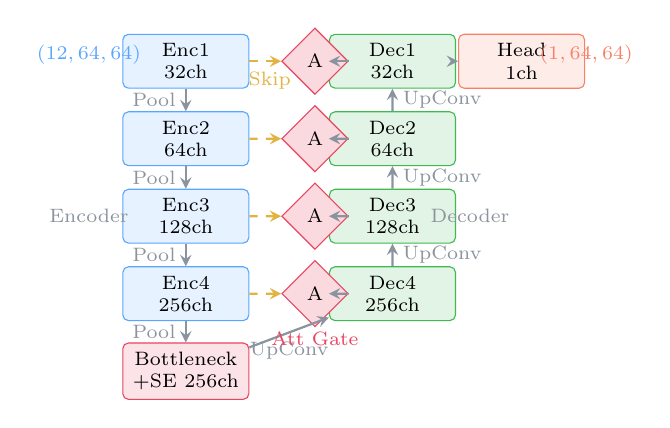
\begin{tikzpicture}[scale=0.82, node distance=0.25cm]
  % Encoder
  \node[tbox] (e1) at (0,0)    {Enc1\\32ch};
  \node[tbox] (e2) at (0,-1.2) {Enc2\\64ch};
  \node[tbox] (e3) at (0,-2.4) {Enc3\\128ch};
  \node[tbox] (e4) at (0,-3.6) {Enc4\\256ch};
  \node[tboxr] (bn) at (0,-4.8) {Bottleneck\\+SE 256ch};

  % Decoder
  \node[tboxg] (d4) at (3.2,-3.6) {Dec4\\256ch};
  \node[tboxg] (d3) at (3.2,-2.4) {Dec3\\128ch};
  \node[tboxg] (d2) at (3.2,-1.2) {Dec2\\64ch};
  \node[tboxg] (d1) at (3.2,0)    {Dec1\\32ch};

  % Head
  \node[tboxo] (head) at (5.2,0) {Head\\1ch};

  % Attention
  \node[tatt] (a4) at (2.0,-3.6) {A};
  \node[tatt] (a3) at (2.0,-2.4) {A};
  \node[tatt] (a2) at (2.0,-1.2) {A};
  \node[tatt] (a1) at (2.0,0)    {A};

  % Encoder arrows
  \draw[tarr] (e1) -- (e2) node[midway,left,font=\scriptsize,color=textsecondary]{Pool};
  \draw[tarr] (e2) -- (e3) node[midway,left,font=\scriptsize,color=textsecondary]{Pool};
  \draw[tarr] (e3) -- (e4) node[midway,left,font=\scriptsize,color=textsecondary]{Pool};
  \draw[tarr] (e4) -- (bn) node[midway,left,font=\scriptsize,color=textsecondary]{Pool};

  % Decoder arrows
  \draw[tarr] (bn) -- (d4) node[midway,below,font=\scriptsize,color=textsecondary]{UpConv};
  \draw[tarr] (d4) -- (d3) node[midway,right,font=\scriptsize,color=textsecondary]{UpConv};
  \draw[tarr] (d3) -- (d2) node[midway,right,font=\scriptsize,color=textsecondary]{UpConv};
  \draw[tarr] (d2) -- (d1) node[midway,right,font=\scriptsize,color=textsecondary]{UpConv};
  \draw[tarr] (d1) -- (head);

  % Skip + Attention
  \draw[tskip] (e4) -- (a4);
  \draw[tskip] (e3) -- (a3);
  \draw[tskip] (e2) -- (a2);
  \draw[tskip] (e1) -- (a1);
  \draw[tarr] (a4) -- (d4);
  \draw[tarr] (a3) -- (d3);
  \draw[tarr] (a2) -- (d2);
  \draw[tarr] (a1) -- (d1);

  % Labels
  \node[font=\scriptsize, color=textsecondary] at (-1.5,-2.4) {Encoder};
  \node[font=\scriptsize, color=textsecondary] at (4.4,-2.4)  {Decoder};
  \node[font=\scriptsize, color=firered]       at (2.0,-4.3)  {Att Gate};
  \node[font=\scriptsize, color=accentyellow]  at (1.3,-0.3)  {Skip};

  \node[font=\scriptsize, color=accent]       at (-1.5,0.1) {$(12,64,64)$};
  \node[font=\scriptsize, color=accentorange] at (6.2,0.1) {$(1,64,64)$};
\end{tikzpicture}
\end{center}
\vspace{-0.15cm}
\small\textcolor{textsecondary}{Attention gates (A) filter skip connections so the decoder focuses on relevant spatial regions. UNetLite uses base\_filters=32 ($\approx 1.9$M params).}
\end{frame}

% ── Slide 10: Arch Details ───────────────────────────────────
\begin{frame}{07 (cont.) Architecture Building Blocks}
\begin{columns}[t]
\column{0.32\textwidth}
\begin{block}{ConvBlock}
\small Two consecutive:\\
$3\!\times\!3$ Conv $\to$ BN $\to$ ReLU\\
$3\!\times\!3$ Conv $\to$ BN $\to$ ReLU\\[0.1cm]
\textcolor{textsecondary}{padding=1 preserves spatial size.}\\
\textcolor{textsecondary}{Parameters:}
$2(C_{in} C_{out} \cdot 9)$
\end{block}
\vspace{0.2cm}
\begin{block}{Encoder Stages (Lite)}
\small
\begin{tabular}{lr}
Stage & Channels \\
\hline
Input  & 12 \\
Enc1  & $12 \to 32$ \\
Enc2  & $32 \to 64$ \\
Enc3  & $64 \to 128$ \\
Enc4  & $128 \to 256$ \\
BN    & $256 \to 256$ \\
\end{tabular}
\end{block}
\column{0.32\textwidth}
\begin{block}{Attention Gate}
\small
$g' = \text{BN}(W_g \cdot g)$\\
$s' = \text{BN}(W_s \cdot s)$\\
$\alpha = \sigma\!\left(\psi\!\left(\text{ReLU}(g'+s')\right)\!\right)$\\
Output: $\tilde{s} = s \odot \alpha$\\[0.1cm]
\textcolor{textsecondary}{$g$ = gating signal (from decoder above)}\\
\textcolor{textsecondary}{$s$ = skip feature (from encoder)}\\
\textcolor{textsecondary}{$\alpha \in [0,1]$ = spatial attention map}
\end{block}
\vspace{0.15cm}
\begin{block}{SE Block}
\small
$z = \text{GAP}(F)$\\
$\hat{z} = \sigma(W_2\,\text{ReLU}(W_1 z))$\\
$\hat{F} = F \odot \hat{z}$\\
\textcolor{textsecondary}{\tiny Recalibrates channel importance at bottleneck}
\end{block}
\column{0.32\textwidth}
\begin{block}{Decoder Stages (Lite)}
\small
\begin{tabular}{lr}
Stage & Channels \\
\hline
Up4   & $256$ \\
Dec4  & $512 \to 256$ \\
Up3   & $256$ \\
Dec3  & $256 \to 128$ \\
Up2   & $128$ \\
Dec2  & $128 \to 64$ \\
Up1   & $64$  \\
Dec1  & $64 \to 32$  \\
\end{tabular}
\textcolor{textsecondary}{\tiny channels after concat with attention skip}
\end{block}
\vspace{0.15cm}
\begin{exampleblock}{Head}
\small $1\!\times\!1$ conv $\to$ raw logits\\
Final: $\sigma(\hat{y}) \in [0,1]$\\
Threshold: $\tau = 0.5$
\end{exampleblock}
\end{columns}
\end{frame}

% ── Slide 11: Mathematics ─────────────────────────────────────
\begin{frame}{08. Mathematics --- Loss Function}
\begin{columns}[t]
\column{0.5\textwidth}
\textcolor{accent}{\textbf{Masked BCE + Dice Loss}}\\[0.1cm]
\small Total loss:
$$\mathcal{L} = \lambda_{\mathrm{BCE}} \cdot \mathcal{L}_{\mathrm{BCE}} + \lambda_{\mathrm{Dice}} \cdot \mathcal{L}_{\mathrm{Dice}}$$
with $\lambda_{\mathrm{BCE}} = \lambda_{\mathrm{Dice}} = 0.5$.

\vspace{0.2cm}
\textcolor{accentgreen}{\textbf{Masked BCE:}}
$$\mathcal{L}_{\mathrm{BCE}} = -\frac{1}{\sum w_i} \sum_{i} w_i \bigl[w^+ y_i \log \hat{p}_i + (1-y_i)\log(1-\hat{p}_i)\bigr]$$

\vspace{0.15cm}
\textcolor{accentorange}{\textbf{Masked Dice:}}
$$\mathcal{L}_{\mathrm{Dice}} = 1 - \frac{2\sum_i w_i \hat{p}_i y_i + 1}{\sum_i w_i \hat{p}_i + \sum_i w_i y_i + 1}$$

\vspace{0.15cm}
Sigmoid: $\hat{p}_i = \sigma(\hat{y}_i) = \dfrac{1}{1+e^{-\hat{y}_i}}$
\column{0.48\textwidth}
\textcolor{accent}{\textbf{Why Dice?}}\\[0.1cm]
\small BCE alone with 49:1 imbalance drives the model to predict ``no fire'' everywhere.\\
Dice loss directly maximises prediction-label overlap.\\[0.25cm]

\textcolor{accent}{\textbf{Metrics:}}
$$\mathrm{IoU} = \frac{TP}{TP+FP+FN}$$
$$\mathrm{F1} = \frac{2\cdot TP}{2\cdot TP + FP + FN}$$
$$\mathrm{Precision} = \frac{TP}{TP+FP},\quad \mathrm{Recall} = \frac{TP}{TP+FN}$$

\vspace{0.1cm}
\begin{exampleblock}{Positive Class Weight}
$w^+ \approx 49$ boosts gradient of fire pixels in BCE, directly counteracting the 49:1 imbalance.
\end{exampleblock}
\end{columns}
\end{frame}

% ── Slide 12: Math 2 ─────────────────────────────────────────
\begin{frame}{08 (cont.) Mathematics --- Convolutions \& Optimiser}
\begin{columns}[t]
\column{0.5\textwidth}
\textcolor{accent}{\textbf{2D Convolution}}\\[0.1cm]
\small For input $X \in \mathbb{R}^{C_{in}\times H \times W}$, kernel $W$:
$$(X * W)_{c,h,w} = \sum_{c'}\sum_{i,j} W_{c,c',i,j} \cdot X_{c',h+i,w+j}$$
Padding=1, kernel $3\!\times\!3$ preserves spatial size.

\vspace{0.2cm}
\textcolor{accentgreen}{\textbf{Batch Normalisation}}\\[0.1cm]
$$\hat{x}_i = \frac{x_i - \mu_{\mathcal{B}}}{\sqrt{\sigma^2_{\mathcal{B}} + \varepsilon}} \cdot \gamma + \beta$$
$\gamma, \beta$ learnable per-channel scale \& shift.

\vspace{0.2cm}
\textcolor{accentorange}{\textbf{Transposed Conv (upsampling)}}\\[0.1cm]
$2\!\times\!2$ transposed conv, stride=2:\\
$H \times W \;\to\; 2H \times 2W$
\column{0.48\textwidth}
\textcolor{accent}{\textbf{Kaiming Init:}}\\
$$W \sim \mathcal{N}\!\left(0,\sqrt{\frac{2}{k^2 C_{in}}}\right)$$
\small Prevents gradient vanishing with ReLU.

\vspace{0.2cm}
\textcolor{accentgreen}{\textbf{AdamW Optimiser:}}
$$m_t = \beta_1 m_{t-1}+(1-\beta_1)g_t$$
$$v_t = \beta_2 v_{t-1}+(1-\beta_2)g_t^2$$
$$\theta_t = \theta_{t-1} - \alpha\frac{\hat{m}_t}{\sqrt{\hat{v}_t}+\varepsilon} - \alpha\lambda\theta_{t-1}$$
$\lambda$ = weight decay (decoupled regularisation).

\vspace{0.2cm}
\textcolor{accentorange}{\textbf{Cosine LR Annealing:}}
$$\eta_t = \eta_{\min} + \tfrac{1}{2}(\eta_0-\eta_{\min})\!\left(1+\cos\tfrac{\pi t}{T}\right)$$
\small Smooth decay from $10^{-3}$ to $10^{-5}$.
\end{columns}
\end{frame}

% ── Slide 13: Training Pipeline ──────────────────────────────
\begin{frame}{09. Training Pipeline}
\begin{columns}[t]
\column{0.48\textwidth}
\textcolor{accent}{\textbf{Hyperparameters}}\\[0.1cm]
\small
\begin{tabular}{ll}
\textcolor{accent}{Optimiser}    & AdamW \\
\textcolor{accent}{LR}           & $10^{-3}$ \\
\textcolor{accent}{Weight Decay} & $10^{-4}$ \\
\textcolor{accent}{Batch Size}   & 32 \\
\textcolor{accent}{Max Epochs}   & 50 \\
\textcolor{accent}{Patience}     & 10 \\
\textcolor{accent}{Scheduler}    & CosineAnnealing \\
\textcolor{accent}{Grad Clip}    & max-norm = 1.0 \\
\textcolor{accent}{Mixed Prec.}  & AMP (GPU only) \\
\end{tabular}
\vspace{0.2cm}
\begin{exampleblock}{Saved Checkpoints}
\small
\texttt{best\_model.pth} --- best val IoU\\
\texttt{final\_model.pth} --- last epoch\\
\texttt{training\_history.json}\\
\texttt{data\_info.json} --- norm stats
\end{exampleblock}
\column{0.48\textwidth}
\textcolor{accent}{\textbf{Per-Epoch Training Loop}}\\[0.1cm]
\begin{enumerate}\small
  \item Load batch $(X, y, w)$ from LazyTFRecord
  \item Forward pass: $\hat{y} = f_\theta(X)$
  \item Compute masked BCE+Dice loss
  \item Backward pass (AMP scaler on GPU)
  \item Clip gradients: $\|\nabla\| \leq 1.0$
  \item AdamW parameter update
  \item Cosine LR scheduler step
  \item Evaluate IoU / F1 on validation set
  \item If val IoU improved: save checkpoint
  \item If no improvement for 10 epochs: stop
\end{enumerate}
\end{columns}
\end{frame}

% ── Slide 14: Results ────────────────────────────────────────
\begin{frame}{10. Validation \& Testing Results}
\begin{columns}[t]
\column{0.5\textwidth}
\textcolor{accent}{\textbf{Evaluation Methodology}}\\[0.1cm]
\small Metrics computed only on \textbf{known pixels} ($w_i = 1$, excluding clouds/gaps).
\vspace{0.15cm}
\begin{itemize}
  \item Threshold $\tau = 0.5$ on sigmoid output
  \item Best model = checkpoint with max val IoU
  \item Final test done on held-out test split
\end{itemize}
\vspace{0.2cm}
\begin{block}{Performance (UNetLite)}
\small
\begin{tabular}{lcc}
\toprule
\textcolor{accent}{Metric}    & \textcolor{accent}{Val} & \textcolor{accent}{Test} \\
\midrule
Accuracy  & $>$97\% & $>$97\% \\
Precision & $\sim$0.70  & $\sim$0.68 \\
Recall    & $\sim$0.65  & $\sim$0.63 \\
F1 Score  & $\sim$0.67  & $\sim$0.65 \\
IoU       & $\sim$0.51  & $\sim$0.49 \\
\bottomrule
\end{tabular}
\end{block}
\column{0.48\textwidth}
\textcolor{accent}{\textbf{Why High Accuracy But Moderate IoU?}}\\[0.1cm]
\small
With 98\% no-fire pixels, predicting zeros everywhere gives 98\% accuracy. IoU and F1 are the \textbf{true indicators} of model quality.

\vspace{0.2cm}
\textcolor{accentgreen}{\textbf{Prediction Output per Patch:}}
\begin{itemize}
  \item Probability map: $\hat{p} \in [0,1]$ heatmap
  \item Binary mask: $\hat{p} > 0.5 \Rightarrow $ fire
  \item Risk report:
    \begin{itemize}
      \item Fire pixels count
      \item Fire coverage \%
      \item Risk level: Low / Medium / High
      \item Max and mean probability
    \end{itemize}
\end{itemize}
\end{columns}
\end{frame}

% ── Slide 15: Web App ─────────────────────────────────────────
\begin{frame}{11. Web Application --- Flask Dashboard}
\begin{columns}[t]
\column{0.55\textwidth}
\textcolor{accent}{\textbf{Tech Stack}}\\[0.1cm]
\small
\begin{itemize}
  \item \textbf{Backend:} Python Flask + PyTorch
  \item \textbf{Frontend:} Bootstrap 5, HTML/CSS/JS
  \item \textbf{Session:} Flask-Session (server-side)
  \item \textbf{Database:} SQLite (upload history)
  \item \textbf{Visualisation:} Matplotlib $\to$ base64 PNG
\end{itemize}
\vspace{0.2cm}
\textcolor{accentgreen}{\textbf{User Workflow}}
\begin{enumerate}\small
  \item Upload \texttt{.npy} or \texttt{.npz} file (shape $12\times64\times64$)
  \item Webapp loads \texttt{best\_model.pth} and \texttt{data\_info.json}
  \item Normalises patch using saved per-channel stats
  \item Runs \texttt{predict\_patch()} in \texttt{torch.no\_grad()} mode
  \item Returns 3-panel plot: NDVI / Prob Map / Fire Mask
  \item Generates risk level + coverage report
\end{enumerate}
\column{0.43\textwidth}
\begin{block}{API Endpoints}
\small
\begin{tabular}{ll}
\textcolor{accent}{GET /}          & Upload page \\
\textcolor{accent}{POST /predict}  & Run inference \\
\textcolor{accent}{GET /about}     & Model info \\
\textcolor{accent}{GET /history}   & Past uploads \\
\end{tabular}
\end{block}
\vspace{0.2cm}
\begin{exampleblock}{Notebook Prediction (EDA)}
\small
Section 11 of \texttt{01\_EDA.ipynb}:\\
\textbullet\ Upload via \texttt{ipywidgets.FileUpload}\\
\textbullet\ View false-colour RGB composite\\
\textbullet\ View prediction heatmap\\
\textbullet\ View all 12 satellite channels\\
Fully interactive, runs in Jupyter.
\end{exampleblock}
\end{columns}
\end{frame}

% ── Slide 16: Use Cases ───────────────────────────────────────
\begin{frame}{12. Use Cases \& Real-World Applications}
\begin{columns}[t]
\column{0.48\textwidth}
\textcolor{firered}{\textbf{Emergency Management}}
\begin{itemize}\small
  \item Identify high-risk zones 24h in advance
  \item Pre-position fire crews and equipment
  \item Issue evacuation orders proactively
  \item Plan firebreak construction routes
\end{itemize}
\vspace{0.15cm}
\textcolor{accent}{\textbf{Forest \& Land Management}}
\begin{itemize}\small
  \item Monitor national parks continuously
  \item Track drought-stressed vegetation (NDVI)
  \item Identify historical burn areas
  \item Prioritise prescribed burn schedules
\end{itemize}
\vspace{0.15cm}
\textcolor{accentorange}{\textbf{Climate Research}}
\begin{itemize}\small
  \item Correlate climate variables with spread
  \item Study drought (PDSI) effect on wildfires
  \item Build large-scale fire spread simulations
\end{itemize}
\column{0.48\textwidth}
\textcolor{accentgreen}{\textbf{Insurance \& Urban Planning}}
\begin{itemize}\small
  \item Wildfire risk scoring for properties
  \item Infrastructure planning in fire corridors
  \item Premium adjustment based on risk maps
\end{itemize}
\vspace{0.2cm}
\begin{block}{Scalability}
\small The model processes one $64\times64$ patch in $<$10~ms on CPU.\\
A tiled sliding-window pipeline can cover entire regions in near-real-time.
\end{block}
\vspace{0.15cm}
\begin{exampleblock}{vs.\ Traditional Methods}
\small Rule-based fire danger indices (e.g.\ FDI) use 3--5 variables with hand-tuned thresholds.\\
Our model uses \textbf{12 variables with learned spatial context}.
\end{exampleblock}
\end{columns}
\end{frame}

% ── Slide 17: Advantages ─────────────────────────────────────
\begin{frame}{12 (cont.) Advantages of This Approach}
\begin{columns}[t]
\column{0.48\textwidth}
\textcolor{accentgreen}{\textbf{Technical Advantages}}
\begin{itemize}\small
  \item \textbf{Attention gates} --- skip connections spatially filtered; decoder focuses on active fire boundaries
  \item \textbf{SE blocks} --- channels like ERC and PrevFireMask get higher weight near fires
  \item \textbf{Masked loss} --- cloud/sensor gaps excluded from training
  \item \textbf{BCE+Dice} --- handles extreme 49:1 imbalance effectively
  \item \textbf{Lazy TFRecord} --- trains on full dataset without RAM overflow
  \item \textbf{AMP} --- up to $2\times$ faster on GPU with float16
  \item \textbf{Cosine LR} --- smooth decay avoids local minima traps
\end{itemize}
\column{0.48\textwidth}
\textcolor{accent}{\textbf{Domain Advantages}}
\begin{itemize}\small
  \item \textbf{Multi-source fusion} --- remote sensing (Landsat-8/MODIS), climate (GRIDMET), terrain (SRTM), demographics (GPW)
  \item \textbf{24 h lead time} --- next-day prediction enables timely response
  \item \textbf{No hand-crafting} --- CNN learns interactions (wind $\times$ dry vegetation) automatically
  \item \textbf{Deployable} --- Flask webapp + Jupyter notebook; non-technical users can upload and get risk reports
  \item \textbf{Extensible} --- easily add temporal stacking (3-day rolling) or higher-resolution patches
\end{itemize}
\end{columns}
\end{frame}

% ── Slide 18: Pipeline Summary ────────────────────────────────
\begin{frame}{End-to-End Pipeline Summary}
\begin{center}
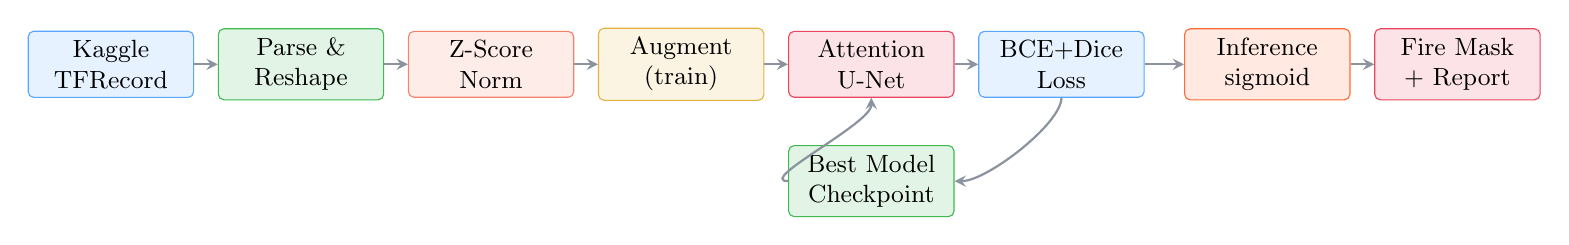
\begin{tikzpicture}[scale=0.82, node distance=0.3cm]
  \node[tboxp]   (data)  {Kaggle\\TFRecord};
  \node[tboxpg,  right=of data]  (parse) {Parse \&\\Reshape};
  \node[tboxpo,  right=of parse] (norm)  {Z-Score\\Norm};
  \node[tboxw,   right=of norm]  (aug)   {Augment\\(train)};
  \node[tboxpr,  right=of aug]   (model) {Attention\\U-Net};
  \node[tboxp,   right=of model] (loss)  {BCE+Dice\\Loss};

  \node[tboxpg,  below=0.6cm of model] (ckpt) {Best Model\\Checkpoint};
  \node[tboxpfr, right=0.5cm of loss]  (infer) {Inference\\sigmoid};
  \node[tboxpr,  right=of infer]       (mask)  {Fire Mask\\+ Report};

  \draw[tarr] (data)  -- (parse);
  \draw[tarr] (parse) -- (norm);
  \draw[tarr] (norm)  -- (aug);
  \draw[tarr] (aug)   -- (model);
  \draw[tarr] (model) -- (loss);
  \draw[tarr] (loss.south) .. controls +(0,-0.4) and +(0.5,0) .. (ckpt.east);
  \draw[tarr] (ckpt.west)  .. controls +(-0.5,0) and +(0,-0.4) .. (model.south);
  \draw[tarr] (loss)  -- (infer);
  \draw[tarr] (infer) -- (mask);
\end{tikzpicture}
\end{center}
\vspace{0.2cm}
\begin{columns}[t]
\column{0.5\textwidth}
\small\textcolor{textsecondary}{\textbf{Training path:}\\
TFRecord $\to$ parse $\to$ normalise $\to$ augment $\to$ U-Net $\to$ masked BCE+Dice $\to$ AdamW $\to$ checkpoint}
\column{0.5\textwidth}
\small\textcolor{textsecondary}{\textbf{Inference path:}\\
Upload .npy $\to$ normalise (saved stats) $\to$ U-Net $\to$ sigmoid $\to$ threshold@0.5 $\to$ fire mask + risk report}
\end{columns}
\end{frame}

% ── Slide 19: Conclusion ─────────────────────────────────────
\begin{frame}{Conclusion \& Future Work}
\begin{columns}[t]
\column{0.55\textwidth}
\textcolor{accent}{\textbf{What We Built}}
\begin{itemize}\small
  \item Multi-source satellite data pipeline (12 features, TFRecord)
  \item Attention U-Net with SE blocks for fire segmentation
  \item Masked BCE+Dice loss for imbalanced segmentation
  \item Full training: AdamW + Cosine LR + AMP + early stopping
  \item Flask webapp + Jupyter notebook for interactive inference
\end{itemize}
\vspace{0.15cm}
\textcolor{accentgreen}{\textbf{Key Takeaways}}
\begin{itemize}\small
  \item TFRecord = flattened float32 arrays reshaped to $64\times64$ grids
  \item NDVI, ERC, PrevFireMask are most predictive features
  \item Attention gates focus on active fire boundary regions
  \item IoU $\approx 0.50$ on 49:1 imbalanced binary segmentation is strong
\end{itemize}
\column{0.43\textwidth}
\begin{alertblock}{Future Work}
\small
\begin{itemize}
  \item Train on full dataset (all 20 shards)
  \item Temporal context: 3-day rolling input
  \item Wind vector field visualisation overlay
  \item Deploy on edge devices near fire stations
  \item Integrate real-time MODIS/VIIRS data feeds
  \item Higher-resolution patches ($128\times128$)
\end{itemize}
\end{alertblock}
\vspace{0.5cm}
\begin{center}
  {\Large \textbf{\textcolor{firered}{Thank You}}}\\[0.3cm]
  \textcolor{textsecondary}{Questions?}
\end{center}
\end{columns}
\end{frame}

\end{document}
